\chapter{Synthetic Experiments}
\label{sec:synthetic}

\subsection{Example datasets}

This section presents the results obtained after learning the datasets introduced in the examples for each model. In every instance 1000 samples were generated from the specific distribution, along with 2000 noise samples ($\nu = 2$). This shows the ability of NCE to learn models that incorporate diversity and coherence between items and features.

\subsubsection{FLID: Two landmarks}

Firstly, recall the following characteristics about the dataset in the example:

\begin{itemize}
  \item There are 3 elements, $h$, $s$, $f$.
  \item There are only 2 possible sets, $\{h,s\}$ and $\{h,f\}$. Both equally likely, i.e. $P(S) = 0.5$.
  \item The model can be realized with a single diversity dimension, i.e. $L=1$.
\end{itemize}

The resulting utility vector and weight matrix are:

\begin{align*}
  \mathbf{u} = \left(5.42,2.82,2.79\right)^{\intercal} \\
  \mathbf{W}^{b} = \left(0.02, 6.10, 6.10\right)^{\intercal}
\end{align*}

This is a slightly different model from the one suggested in section \ref{sec:flid-toy}, however the normalized probability distribution for this model shown in table \ref{tab:flid-toy-learned-probs} proves that it closely approximates the distribution.

\begin{table}
  \centering
  \caption{Learned distribution for example \ref{sec:ffldc-toy}}
  \begin{tabular}{@{}ll@{}}
    \toprule
    $S$ & $P(S)$\\
    \midrule
    $\{h,s\}$ & $0.48$ \\
    $\{h,f\}$ & $0.47$ \\
    $\{h\}$ & $0.03$ \\
    $\{h,s,f\}$ & $0.02$ \\
    \bottomrule
  \end{tabular}
  \label{tab:flid-toy-learned-probs}
\end{table}

\subsubsection{FLDC: Disjoint pairs}

Firstly, recall the following characteristics about the dataset in the example:

\begin{itemize}
  \item There are 4 items, i.e. $V = \{1,2,3,4\}$.
  \item There are only 2 possible sets, $\{1,2\}$ and $\{3,4\}$. Both equally likely, i.e. $P(S) = 0.5$.
  \item The model can be realized with a 2 diversity and 2 coherence dimensions.
\end{itemize}

Figure \ref{fig:fldc-toy-learned-weights} shows the resulting utility vector $\mathbf{u}$ and weight matrices $\mathbf{W}^{b}, \mathbf{W}^{e}$ after learning.

\begin{figure}
  \centering
  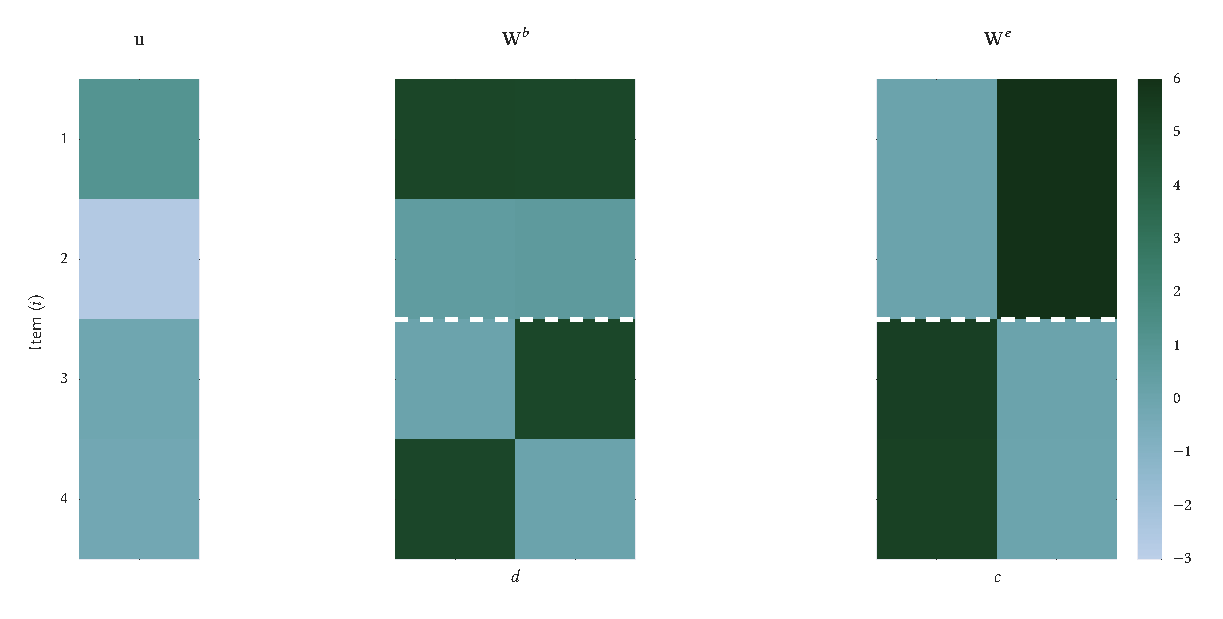
\includegraphics[width=\textwidth]{fldc_toy_example_learned_weights}
  \caption{Learned model for example \ref{sec:fldc-toy}. The white line divides the disjoint pairs described in the example.}
  \label{fig:fldc-toy-learned-weights}
\end{figure}

The model shown in the figure displays the desired properties of diversity between the disjoint pairs whilist having coherence between the items in each pair. Despite being different from the proposed model in section \ref{sec:fldc-toy} it approximately realizes the desired distribution.

\subsubsection{FFLDC: Rated locations}

Firstly, recall the following characteristics about the dataset in the example:

\begin{itemize}
  \item There are 6 items, i.e. $V = \{1,2,3,4,5,6\}$.
  \item The full distribution is related to the features and is given in table \ref{tab:ffldc-toy-probs}.
  \item The proposed model has 2 diversity dimensions and one coherence dimension.
\end{itemize}

\begin{figure}
  \centering
  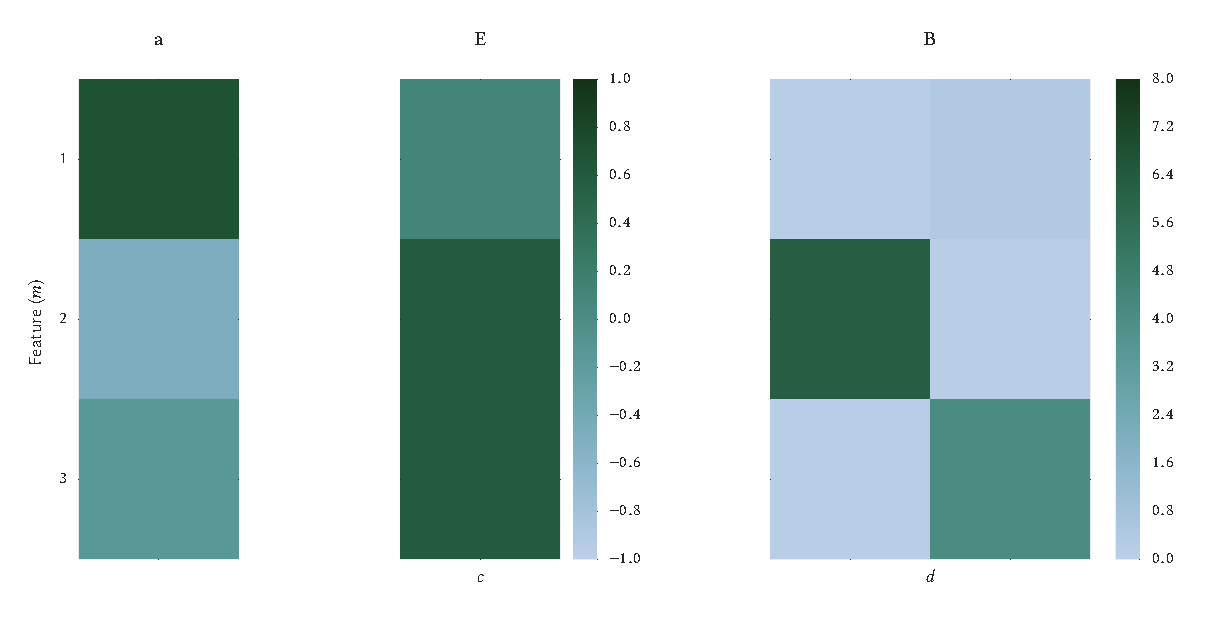
\includegraphics[width=\textwidth]{ffldc_toy_example_learned_weights}
  \caption{Learned model for example \ref{sec:ffldc-toy}}
  \label{fig:ffldc-toy-learned-weights}
\end{figure}

Figure \ref{fig:ffldc-toy-learned-weights} shows the resulting model after learning. Unfortunately, this model can be not as easily interpreted as the one proposed in figure \ref{fig:ffldc-toy-all-weights}, nevertheless it accurately models the distribution from the example. This result demonstrates the ability of the learning algorithm to represent a distribution using features.

It is important to note that the presented results for these experiments correspond to the best of multiple runs. It was observed that the learning algorithm does not always arrive to a good solution. This is explained by the fact that $g(\theta)$ is not a convex function which means that there exists the risk of reaching a local minima in some cases. Due to this, most of the experiments in the following sections are executed over several data folds to account for the randomness.

\subsection{Learning rate sensitivity}

This section expands on the discussion about the learning rate and explores its effect on the learning of the synthetic data from the FFLDC example in section \ref{sec:ffldc-toy}, as well as the effect of implementing AdaGrad.

The first experiment considers the stability of the optimization without AdaGrad. In the experiments presented in this section the following configuration of the learning algorithm is used:

\begin{itemize}
  \item 1000 data samples from the distribution in table \ref{tab:ffldc-toy-probs} are used, along with 2000 noise samples, i.e. $\nu = 2$.
  \item Each run does 100 passes over the data and noise samples.
  \item The algorithm is executed 8 times to obtain statistics about the results.
\end{itemize}

Figure \ref{fig:effects_eta_0} shows the behavior of $g(\theta)$ during learning, each point corresponds to the average value of $g(\theta)$ after each pass over the data and noise samples with its corresponding 95\% confidence interval.

\begin{figure}
  \centering
  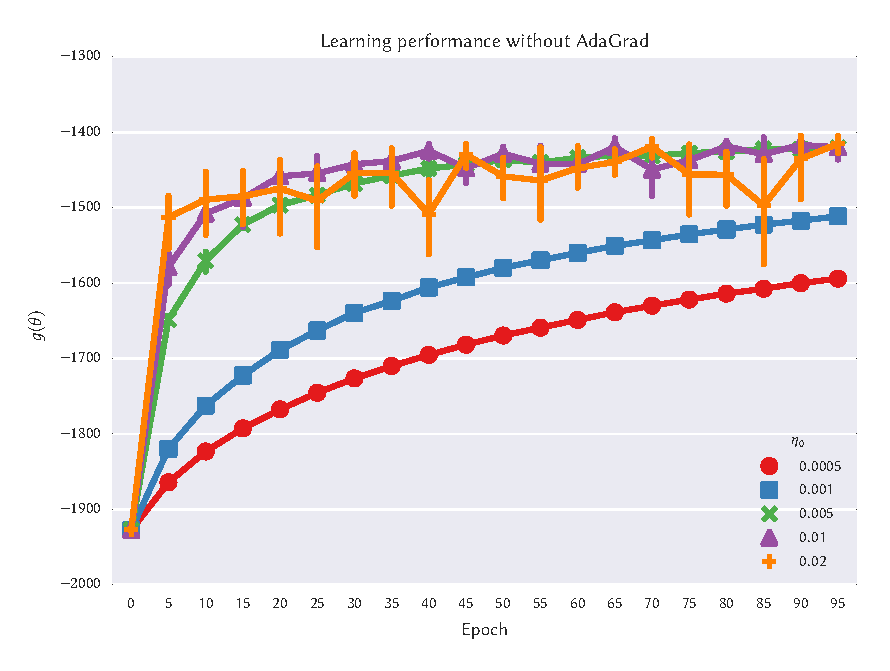
\includegraphics[width=\textwidth]{effects_eta_0_ffldc}
  \caption{Objective function during learning for various values of $\eta_0$ without AdaGrad.}
  \label{fig:effects_eta_0}
\end{figure}

The results in figure \ref{fig:effects_eta_0} display what was mentioned in section \ref{sec:adagrad}, they show that for small values of $\eta_0$ the learning can be significantly slow and that large values of $\eta_0$ may lead to instability. Concretely,  the first row displays slow but stable learning rates while the last row displays learning rates that are too high, the middle row displays the ideal learning rates. Fortunately, in the particular case of this synthetic dataset there exists a learning rate for which the objective function converges however, as it will be seen on real data, this is not always the case. An interesting characteristic shown in this figure is the behavior of the confidence intervals for $\eta_0 = 0.005$, even though the learning is considerably slow there is also a large variation, in this instance the initialization has a larger influence because the learned model doesn't change much from it.

In contrast, figure \ref{fig:effects_adagrad} shows the objective function for various values of $\eta_{0}$ after incorporating AdaGrad to the implementations. These results show that training with AdaGrad is stable for a larger range of $eta_0$, although slower for small values of $\eta_{0}$ which were good for the learning without AdaGrad. For large enough $\eta_0$ values, it can be clearly seen from the figure that SGD with AdaGrad reaches convergence significantly faster, often in the first few iterations.

\begin{figure}
  \centering
  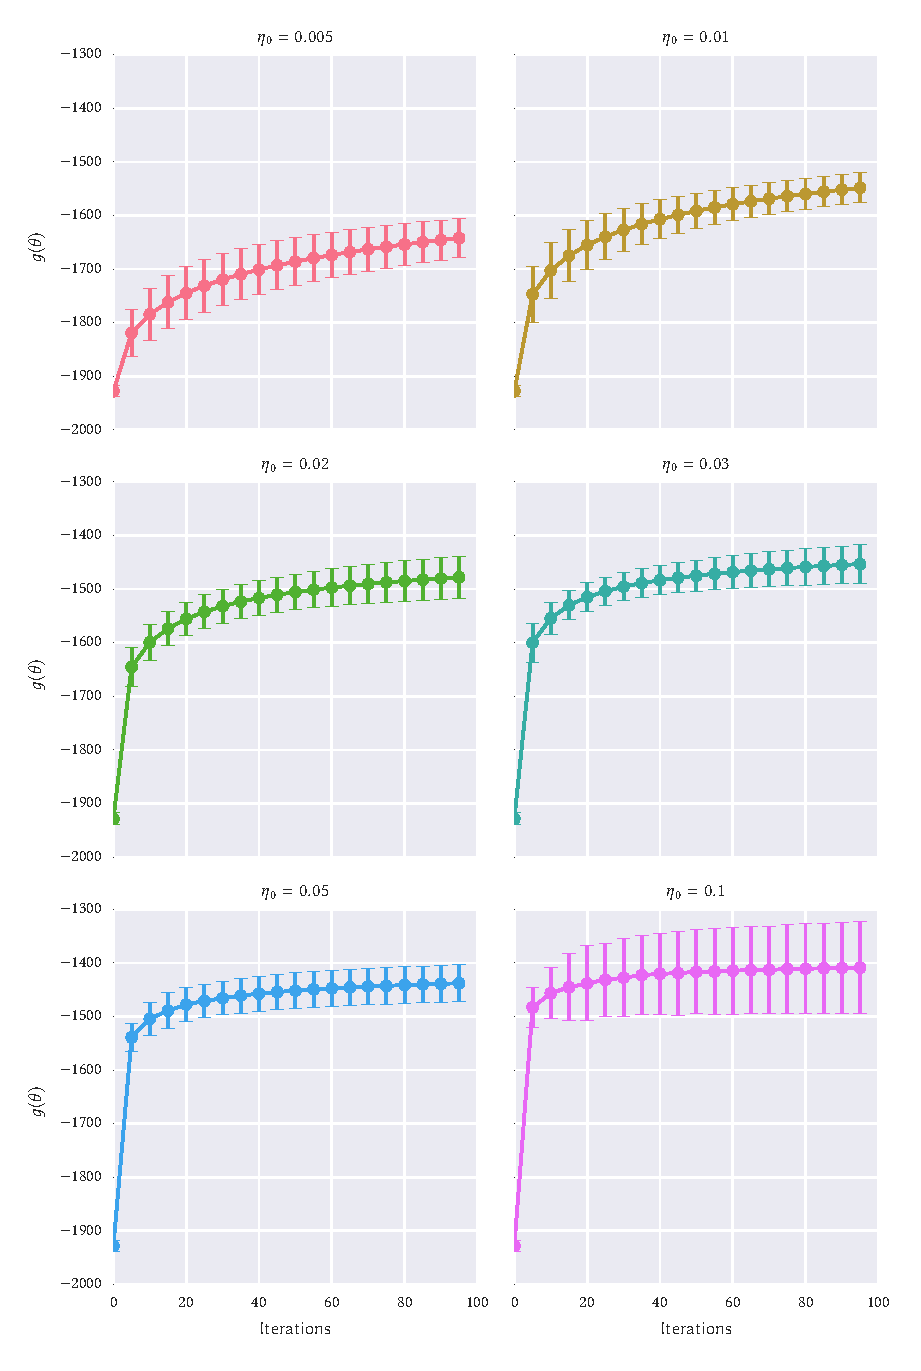
\includegraphics[width=\textwidth]{effects_eta_0_ffldc_adagrad}
  \caption{Objective function during learning for various values of $\eta_0$ with AdaGrad.}
  \label{fig:effects_adagrad}
\end{figure}

Finally, figure \ref{fig:comparison_adagrad_ffldc_toy} shows a direct comparison between training with and without AdaGrad using the best values of $\eta_0$ for each configuration. In this figure both algorithms converge to an optimal value, however it also shows that training with AdaGrad converges significantly faster and its average appears slightly more stable.

These combined results indicate that using AdaGrad is the best strategy for learning the models.

\begin{figure}
  \centering
  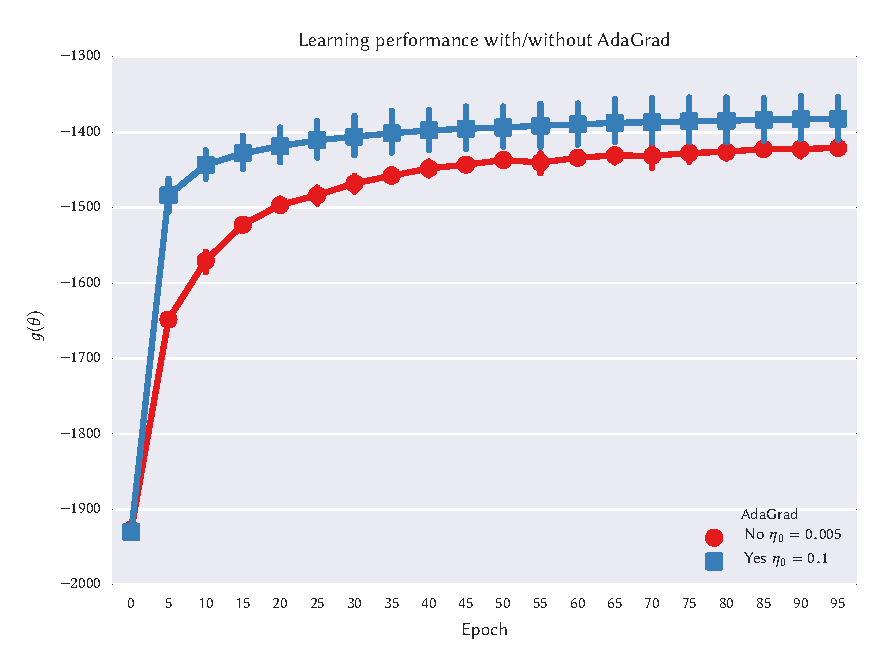
\includegraphics[width=\textwidth]{ffldc_adagrad_comparison}
  \caption{Comparison of learning performance with and without AdaGrad. Initial learning rates are $\eta_0 = 0.05$ with AdaGrad and $\eta_0 = 0.005$ without AdaGrad.}
  \label{fig:comparison_adagrad_ffldc_toy}
\end{figure}

Following the first two suggestions, the noise distribution is sampled from a modular model as the one from equation \ref{eq:modular}. This distribution is constructed from estimated marginals, i.e. $\hat{P}(i \in S)$, which are computed using the maximum likelihood estimator, i.e. $\hat{P}(i \in S) = \nicefrac{\#N(i \in S)}{|\mathcal{D}|}$. Then the utilities for the modular model are given by:

\begin{equation}
u_{i} = \log{\left(\frac{1}{\hat{P}(i \in S)} - 1\right)}
\end{equation}

This model is easy to sample from, hence allowing an efficient generation of large noise samples.